\chapter{The MapReduce paradigm}
This short chapter discusses the MapReduce paradigm, concluding the overview of the problem before exploring the solution proposed by this work. Firstly, a definition and the history of such paradigm will be provided. Then, the programming model will be discussed, explaining the basic concepts needed to utilize MapReduce; following that, an overview of the master-slave architecture is provided. Continuing the chapter, in an attempt to clarify as much as possible how the actual execution of a program that employs MapReduce works, an easy example of a MapReduce computation is displayed. To conclude this chapter, an analysis of the execution flow is presented.

\section{Definition and history}
\textbf{MapReduce} is a \textbf{popular programming model} designed to \textbf{easily process and generate large datasets on clusters of commodity machines}. Through this paradigm, a computation can be expressed in terms of a \textbf{map and reduce functions} while \textbf{the underlying system deals with communication, parallelization and error handling}, making it easy to use even for programmers who have no experience with distributed systems.

\textbf{Google} created this paradigm in \textbf{2003} in order to reduce development time and cost on their projects; after an analysis of the problem, Google's engineers noticed how \textbf{the majority of the computations in their products could be expressed through the map and reduce abstractions} that are typically present in \textbf{functional languages}. The MapReduce paradigm has been \textbf{used in a variety of Google's project}, including the indexing system used by the Google search engine \cite{google_mapreduce}.

\textbf{\href{https://hadoop.apache.org/}{Apache Hadoop}}, inspired by Google's work, integrates the MapReduce paradigm in its free-licensed framework, making it \textbf{one of the most used options} when it comes to applying distributed computations following this paradigm.

\section{The programming model}
In order to execute a MapReduce computation, it is required, as \textbf{input}, \textbf{a set of key/value pairs}. Said values are \textbf{modified through the Map and Reduce functions} and, ultimately, produce as \textbf{output another set of key/value pairs}. 

The Map and Reduce functions are \textbf{written by the user} but in the background, through the framework, behave in the following way:
\begin{itemize}
    \item \textbf{Map}: \textit{(k1, v1) $\Longrightarrow$ list(k2, v2)}\\
    The map function takes a single pair as input and produces a set of intermediate key/value pairs. The framework automatically merges the intermediate sets, grouping them using the keys. Said values are then passed as input to the Reduce function.
    \item \textbf{Reduce}: \textit{(k2, list(v2)) $\Longrightarrow$ list(v2)}\\
    The Reduce function uses the input provided by the automatic merge performed by the framework; every Reduce execution takes a pair of composed of the intermediate key and a collection of values associated to that key. Said pairs are provided using an iterator in order to work with collections that are too large to fit in memory. The values associated to the key are merged to form a possibly smaller set of values, resulting typically in one or zero output values produced as result (even though the function produces a list of values).
\end{itemize}
A programmer that implements a computation following this paradigm does not need to provide anything else but, \textbf{behind the scenes}, the framework performs additional operations such as \textbf{Splitting} (that divides the input in smaller parts to be executed on the multiple workers), \textbf{Shuffling} (that merges the output of the individual Map functions) and \textbf{Collect} (that reunites results produced by the various workers).

Even though the functioning of this paradigm is conceptually easy, the next section analyzes its execution flow with a concrete example.
\section{Architecture}
TODO

\begin{figure}[H]
    \centering
    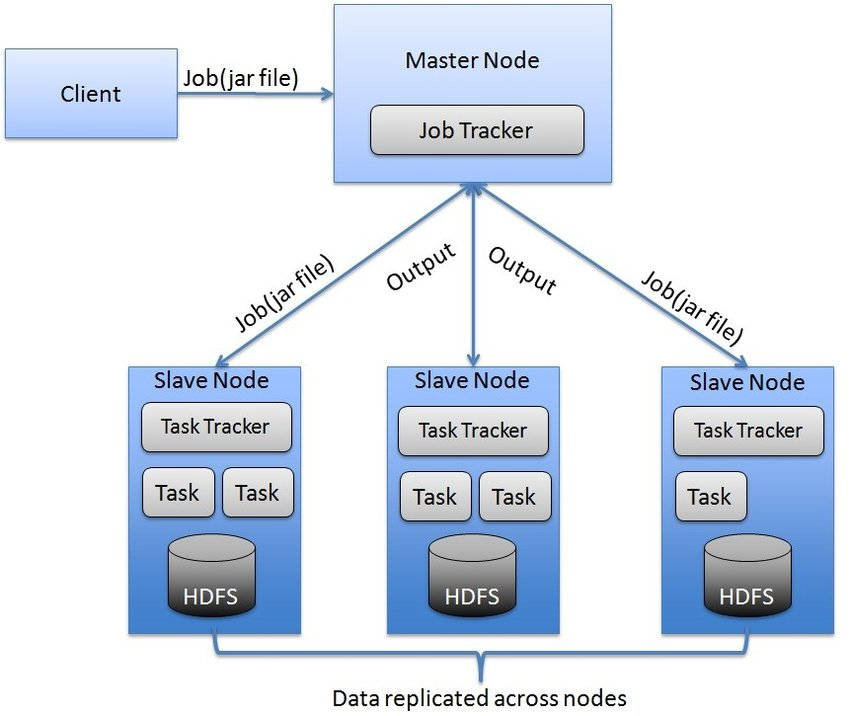
\includegraphics[scale=0.45]{document/chapters/chapter_4/images/hadoop_master_slave_architecture.png}
    \caption{Hadoop's MapReduce master-slave architecture\cite{hadoop_map_reduce}}
    \label{fig:hadoop_master_slave_architecture}
\end{figure}
\section{Example}
In this example (\textit{figure \ref{fig:mapreduce_example}}), a simple word count will be performed: given a source of text, the algorithm will count the occurrences of every word appearing in such text.

\begin{figure}[H]
    \centering
    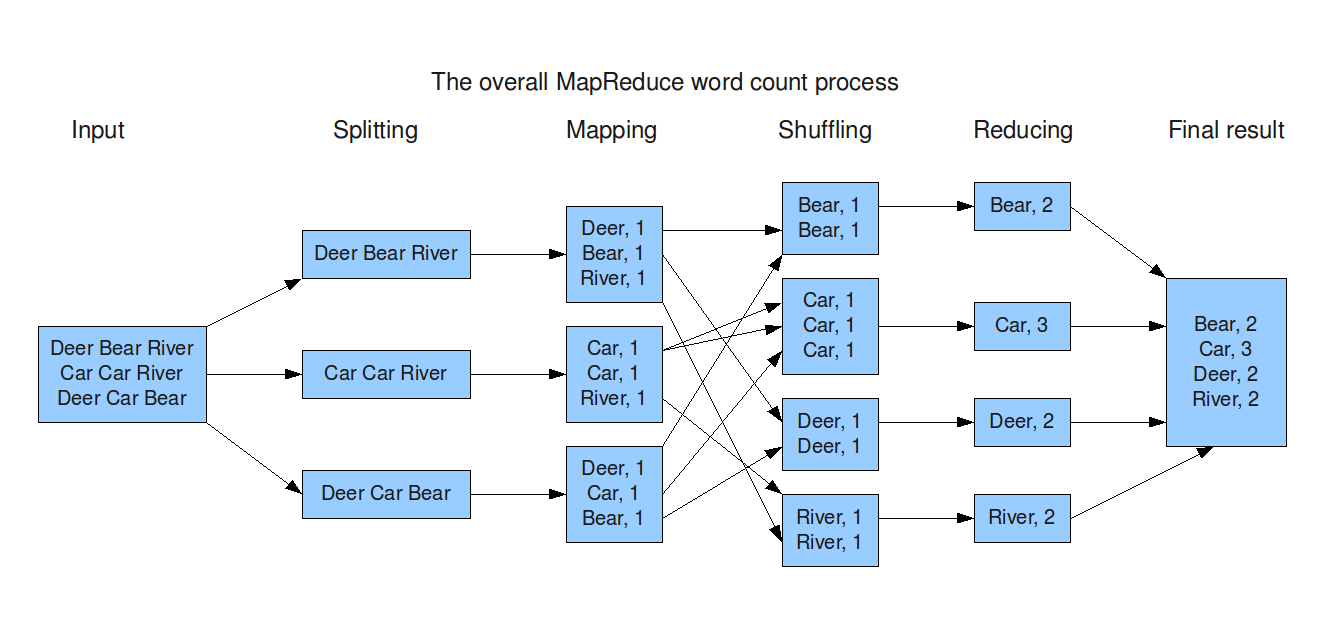
\includegraphics[width=\linewidth]{document/chapters/chapter_4/images/mapreduce_example.png}
    \caption{Example of word count expressed through the MapReduce paradigm \cite{mapreduce_example_site}}
    \label{fig:mapreduce_example}
\end{figure}

The process begins with splitting the input into smaller portions, in this case the text is split by row. On the resulting portions, the Map function is performed; in this example, every word (that is used as a key) is mapped to the value "1" (since it is one appearance of said word). The results are then grouped through the Shuffling operation, using the key as the grouping criteria. Finally, the Reduce function is executed, in different machines, on every group (the example sums the values in order to get the final number of occurrences for every word); the results of the Reduce operations is then collected, obtaining the final collection of key/value pairs.

Even though this example is displayed with a limited quantity of input and output data, the same mechanism can be expanded working with Big Data applications. The key here is the performance augmentation given by parallelizing the execution of the various computational steps across the cluster's machines participating in the MapReduce operation.
\section{Execution flow}
When it comes to understanding the actual flow of execution in a MapReduce cluster, two parameters need to be discussed:
\begin{itemize}
    \item \textit{The number of splits \textbf{M} (Map input)}\\
    This value determinate how many portions the input data will be divided into; this value should be set accordingly to have each portion between 16 and 64 Mb in size.
    \item \textit{The number of intermediate key partitions \textbf{R} (Reduce input)}\\
    The intermediate key space is partitioned into R pieces using a partitioning function (e.g. \textit{hash(key) mod R} \cite{google_mapreduce}), distributing the Reduce invocations. R is usually a small multiple of the number of cluster machines that will be used.
\end{itemize}
The partitioning function, M and R can be set by the user. Typically, MapReduce operations performed at Google have M=200000 and R=5000 with 2000 machines \cite{google_mapreduce}.

The Master, acting as coordinator and intermediary between the Worker nodes, mainly keeps two data structures in memory:
\begin{itemize}
    \item \textbf{Tasks' state}\\
    For every Map task and every Reduce task (for a total number of M + R), the Master keeps track of the current state, that can be either idle, in progress or completed.
    \item \textbf{Intermediate results location}\\
    The master stores the locations and sizes of the R intermediate file regions produced by the map task in order to communicate said data to the Reduce Workers that are in the "in progress" state.
\end{itemize}

\begin{figure}[!ht]
    \centering
    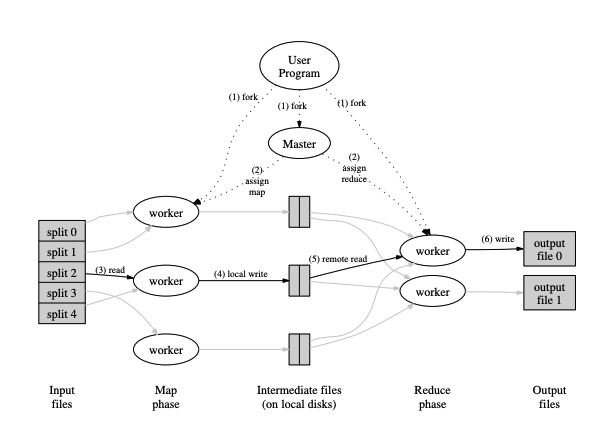
\includegraphics[scale=0.75]{document/chapters/chapter_4/images/mapreduce_execution_flow.png}
    \caption{MapReduce execution flow \cite{google_mapreduce}}
    \label{fig:mapreduce_execution_flow}
\end{figure}

\textit{Figure \ref{fig:mapreduce_execution_flow}} shows an example of execution flow (the enumeration in the following list corresponds to the numeric labels displayed in the figure) with M=5, R=2 and 6 machines (the R parameter has not an optimal value, but this is done only for explanatory reasons):
\begin{enumerate}
    \item The MapReduce library on the User program side splits the input accordingly to the M parameter and starts many copies of the program on the cluster's machines. One of the machines acts as the Master and the others as Workers (\textit{section \ref{map_reduce_architecture}}). The Map and Reduce functions' code is propagated to the machines and the User Program waits to be notified by the Master after the completion of the MapReduce tasks.
    \item The Master assigns the total M + R tasks to the Workers, being a Map task or a Reduce task.
    \item A Worker that executes a Map task reads the corresponding input piece among the M parts. The key/value pairs are processed through in the User-defined Map function and the intermediate results are buffered in memory.
    \item Periodically, the buffered intermediate results are written on the local disk. Said results are partitioned locally in R regions following the partitioning function. After that, the Worker communicates the location of such results to the Master which, in turn, forwards this information to the Reduce Workers.
    \item When a Worker is notified about the availability of new results, it reads them (using the location previously provided) from the correct Workers and, once it has all the data for its region, it sorts such data using the intermediate key, grouping together data that belongs to the same key. If the intermediate data is too large to fit in memory, the sorting is done using the disk.
    \item The Worker iterates over the data and, for each key, performs the Reduce function provided by the User. This produces a file containing all the Reduce results for the region handled by the Worker.
    \item After all the Map and Reduce tasks are completed, the User program is notified, and it can resume its execution.
\end{enumerate}

The final output of the R files can then be accessed as it is, combined into a single source, or used as input for a new MapReduce execution.